%
% The first command in your LaTeX source must be the \documentclass command.
\documentclass[sigchi, authorversion, screen]{acmart}

\settopmatter{printacmref=false} % Removes citation information below abstract
\renewcommand\footnotetextcopyrightpermission[1]{} % removes footnote with conference information in first column
\pagestyle{plain} % removes running headers


\usepackage[utf8]{inputenc}
\usepackage[T1]{fontenc}
\usepackage[french, english]{babel}
\usepackage{caption}
\usepackage{graphics} % for pdf, bitmapped graphics files
\usepackage{graphicx}
\usepackage{subcaption}
\usepackage{hyperref}

%
% defining the \BibTeX command - from Oren Patashnik's original BibTeX documentation.
\def\BibTeX{{\rm B\kern-.05em{\sc i\kern-.025em b}\kern-.08emT\kern-.1667em\lower.7ex\hbox{E}\kern-.125emX}}

\graphicspath{
    {Images/}
}

%
% end of the preamble, start of the body of the document source.
\begin{document}

%
% The "title" command has an optional parameter, allowing the author to define a "short title" to be used in page headers.
\title{AR Spells - An interactive augmented reality game with Microsoft's Hololens and tangible spells}

%
% The "author" command and its associated commands are used to define the authors and their affiliations.
% Of note is the shared affiliation of the first two authors, and the "authornote" and "authornotemark" commands
% used to denote shared contribution to the research.
\author{Dimitri Belopopsky}
\email{dimitri@belopopsky.com}
\affiliation{%
  \institution{Université Paris-Saclay}
}

\author{Adèle Colas}
\email{adele.colas@u-psud.fr}
\affiliation{%
  \institution{Université Paris-Saclay}
}

\author{Emmanuel Courtoux}
\email{e.courtoux@gmail.com}
\affiliation{%
  \institution{Université Paris-Saclay}
}

\author{Matija Veljkovic}
\email{veljkovic.matija@gmail.com}
\affiliation{%
  \institution{Université Paris-Saclay / EIT Digital Academy}
}

\author{Jean-Marc Vezien}
\email{vezien@limsi.fr }
\affiliation{%
  \institution{Université Paris-Sud, Inria, CNRS, Université Paris-Saclay}
}

\author{Anastasia Bezerianos}
\email{anastasia.bezerianos@lri.fr}
\affiliation{%
  \institution{Université Paris-Sud, Inria, CNRS, Université Paris-Saclay}
}



%
% By default, the full list of authors will be used in the page headers. Often, this list is too long, and will overlap
% other information printed in the page headers. This command allows the author to define a more concise list
% of authors' names for this purpose.
\renewcommand{\shortauthors}{AR Spells}

%
% The abstract is a short summary of the work to be presented in the article.
\begin{abstract}
We present AR spells \cite{github-project}, an interactive augmented reality game on Microsoft’s Hololens which combines a tower-defense style game with a crafting system to create spells using tangibles. The goal of our work was to build an augmented reality application with tangible interactions using Hololens. We propose "AR Spells" a game where the user can interact with an augmented reality map by killing the monsters using tangible interaction to create the right spell. The paper retraces the creation of the application from the source of its conception to its technological design. The project was presented during the 2019 exhibition from students of the Master in Human Computer Interaction and Design from the Paris-Saclay University. The evaluation and possible evolution imagined after this exhibition are presented as well.

\end{abstract}


%
% Keywords. The author(s) should pick words that accurately describe the work being
% presented. Separate the keywords with commas.
\keywords{Hololens, augmented reality, video game, tangibles, Unity, markers}

%
% A "teaser" image appears between the author and affiliation information and the body 
% of the document, and typically spans the page. 
  \begin{teaserfigure}
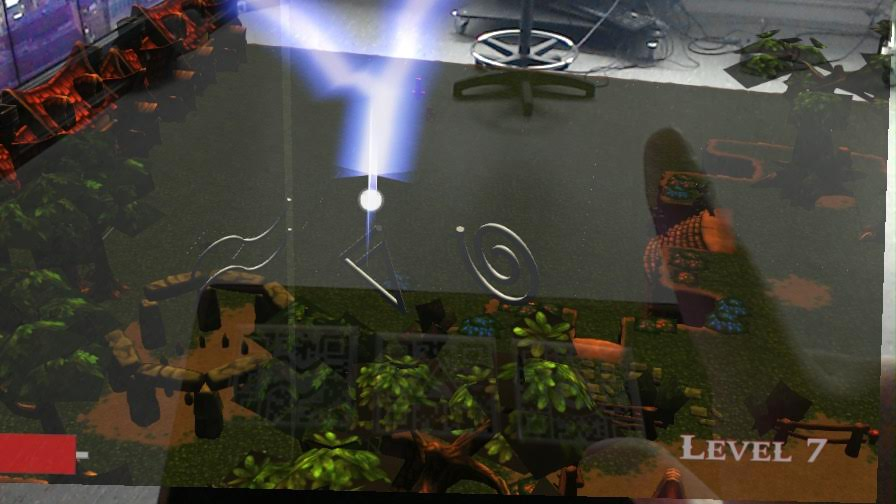
\includegraphics[width=\textwidth]{game_overview.jpg}
  \caption{A snapshot of the game as seen from the Hololens helmet. A spell (lightning) has been crafted with the tangibles and is ready to be used on the monsters.}
  \Description{The Hololens helmet (lower right), the tangibles used for spell crafting (lower left) and a preview of the game in Unity.}
  \label{fig:game_teaser}
\end{teaserfigure}


%
% This command processes the author and affiliation and title information and builds
% the first part of the formatted document.
\maketitle

\section{Introduction}

AR Spells is an Augmented Reality application using tangible interaction. The goal here is to protect a hero from enemies attacking him. With only two types of enemies, the player must select the right spell to defeat them. To select the spell, between fire or lightning see Figure 6, the player must place the tagged tangibles in the right order on the tablet. He then can defeat the enemy by selecting them using the gaze cursor and applying using a pinch gesture used in the Hololens. The project was presented during the 2019 exhibition from students master HCI And Design from the Paris-Saclay University. The feedback given during this exhibition will be highlighted within this paper as well as the process of building the app, its design and and the challenges we faced.

\begin{figure}[ht]
  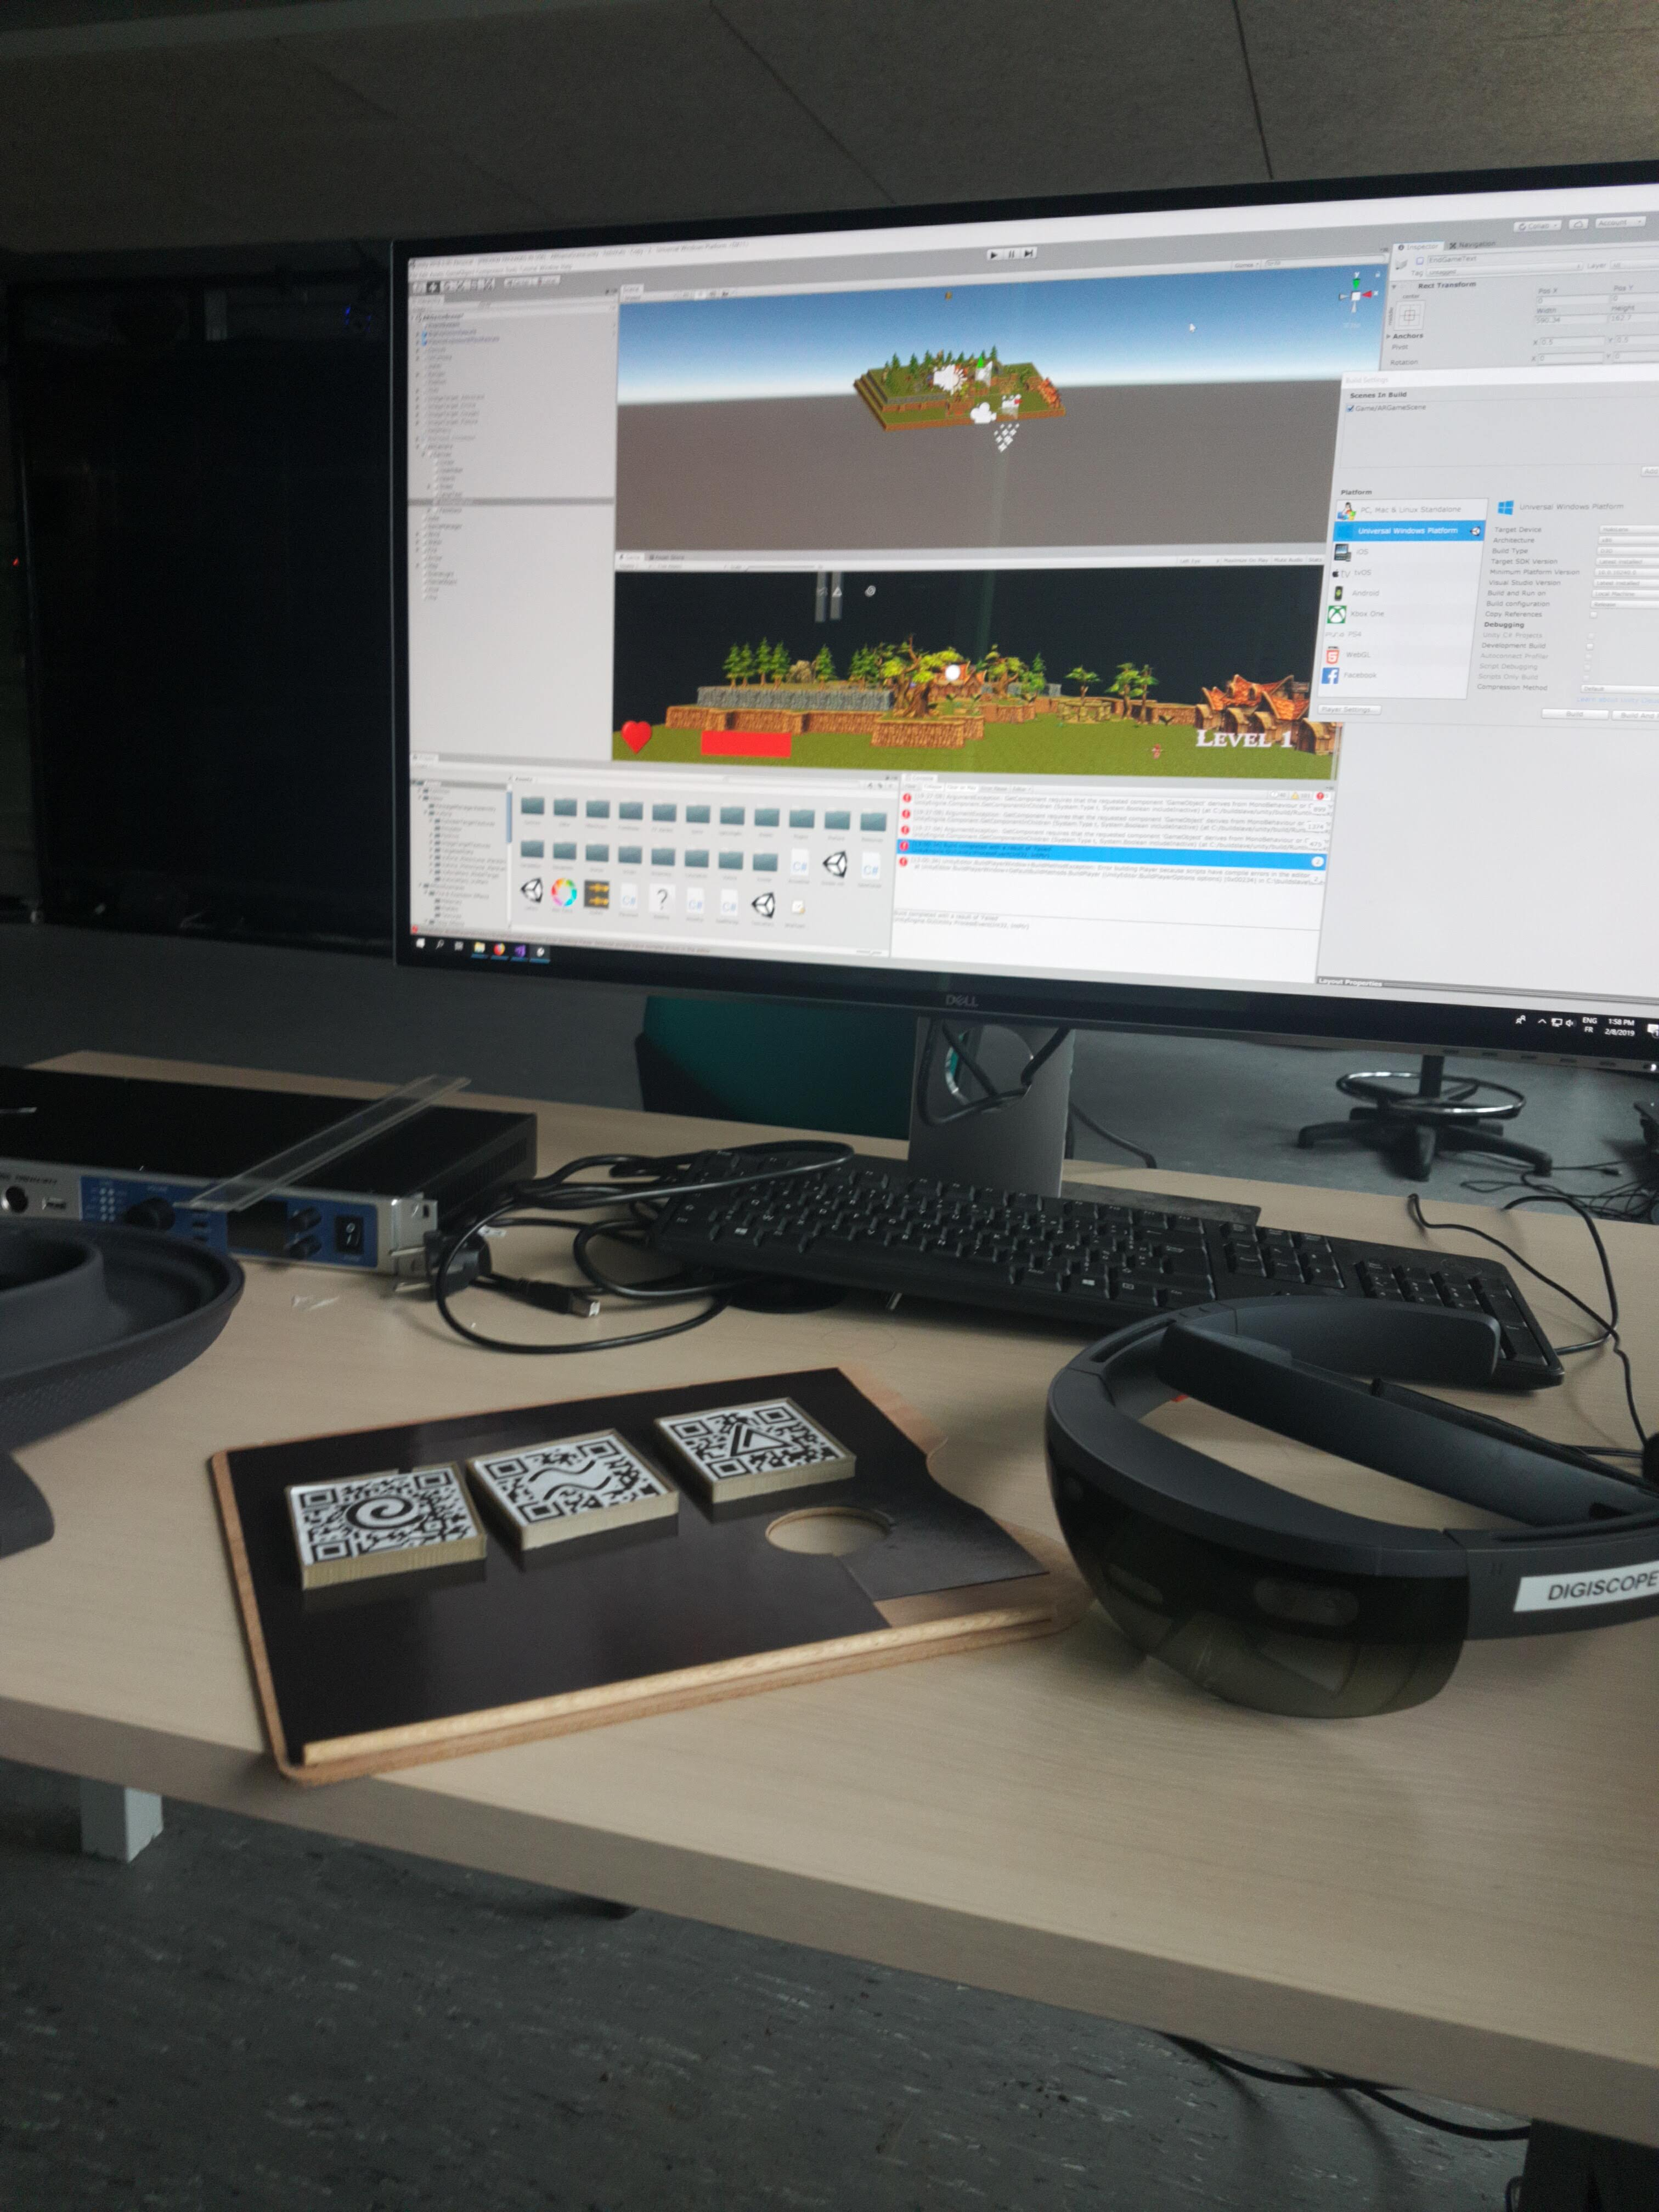
\includegraphics[width=0.4\textwidth]{project_preview.jpg}
  \caption{The Hololens helmet (lower right), the tangibles used for spell crafting (lower left) and a preview of the game in Unity.}
  \Description{The Hololens helmet (lower right), the tangibles used for spell crafting (lower left) and a preview of the game in Unity.}
  \label{fig:setup_teaser}
\end{figure} 

\section{Related Works}

Hado \cite{hado}, is a startup specialised in augmented reality sport/e- sport using augmented reality headsets and smartphones for gesture recognition. It’s designed to be a multiplayer game which runs in a room.

Pokemon GO \cite{pokemongo} is a solo AR game which uses spatial mapping to position the Pokemons on the ground, and requiring to move around the environment to look for them before trying to catch them. This increases engagement and immersion in the game, but requires environment to be well scanned (not too many small objects or details, good lighting, ...) for it to work correctly.

RoboRaid \cite{roboraid}is an augmented reality game developed by Microsoft. It uses spatial mapping to detect a wall, through which robots smash through, and then move around the walls. Your goal is to defend a drone whose AI is being targeted by the robots. 

Several games such as DRAKERZ-Confrontation \cite{drakerz} or Genesis Augmented \cite{genesisaugmented} make use of marker based AR for their games. Those markers are used as anchors in the 3D environment, to realistically place virtual objects and make the virtual avatars interact with each other as though being part of the environment.

AR games tend rely either on spatial mapping and markers, but usually not both. The direct purpose of those technologies is to setup the virtual environment correctly in the real world. Markers can also be used to interact with other markers, but their influence on the environment is more designed for animation and immersion purposes and not influencing that environment (dynamically change it).


\section{System Design}

In this chapter we will cover the technical implementation of the system in detail.

\subsection{Early design}
The basic idea that led to this result was to create an application were the user will be able to combine virtual objects together to make new ones. We thought about cooking recipes as well as color mixing but what resulted of our brainstorming was the spells and a game were the user could use them to accomplish his goal. We had to use tangibles and it looked like using markers to augment them was the right way to go. As said before, we first wanted to make a tower-defense like game were the user had to stop a monster from destroying a city by throwing spells at him. Also, the idea we had for "AR spell" was using more tangible objects. The same map would be used but we would not act directly on the enemies. The idea was to use Vuforia \cite{vuforia} to create tangible marker-based traps. Those traps could be handled by the player and placed on the ground and be dynamically recognized as a virtual game object. That way traps would also be augmented and added to the map so that the characters of the map would react to it. Then the player would have to use the right spell (as he does in the final version). For instance a wall could be activated by the spell "earth" , barrels would explode if fire would be thrown at them and the crossbow’s arrow would be fired with wind (see fig.3). In this idea, we would have much more interactions between virtual object and tangible one. But this idea was just a draw a wasn’t taking in account the tracking possibilities of the Hololens which are limited to a small field of view. The tracking of the trap’s tangible was not satisfying enough, and we had to cut them off the final project creating this way a more direct interaction with the enemies. We also wanted to have some gesture recognition to make the game more immersive. The user being able to grab the spell in the palm of his hand and throw it at the target was one of the original ideas but once again we were limited by the Hololens capabilities in terms of field of view as well as gesture recognition. That’s why our final design only use the basic pinching gesture provided by the Hololens system to interact with the different game object.

\begin{figure}[ht]
  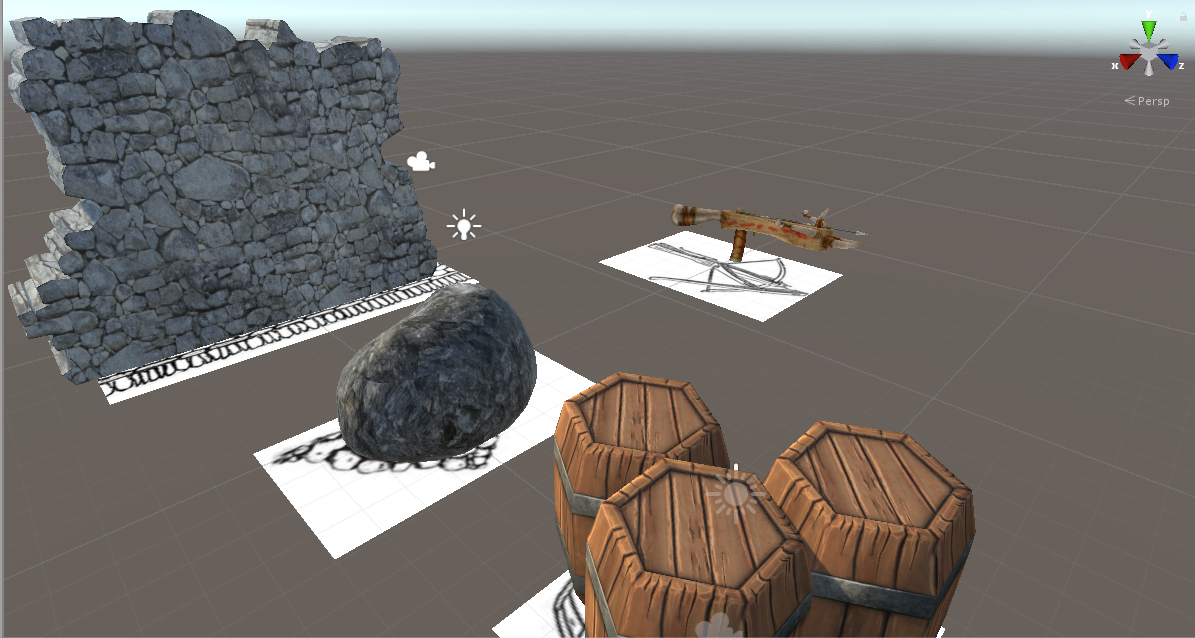
\includegraphics[width=0.4\textwidth]{traps.png}
  \caption{The scene with the augmented traps using Vuforia on Unity}
  \label{fig:traps}
\end{figure}

\subsection{Gameplay} 

For implementing the game itself, a Udemy course was used as guidelines and technical assistance. This is also where the assets were acquired from. Originally, the goal of the course is to make a third player PC game in which you control the hero and fight of the enemies.


\subsection{Creating the map environment}

The map creation was made easier as we had the access to the assets such as the models, materials, textures, etc. Despite that, it still took a significant amount of time to finalize the map we wanted. We needed to combine every- thing so it would look appealing and add the mesh renderers and colliders in order to bake a proper navigation mesh for the AI controlling the enemies. The NavMesh bake (see Figure \ref{fig:navmesh_unity})gave us a lot of problems when we needed to resize everything for the size to fit the one we wanted to have with Hololens and when we needed to spawn enemies dynamically. Other difficulties included the problems with Unity version compatibility being that the assets were used in a much older Unity version.


\begin{figure}
    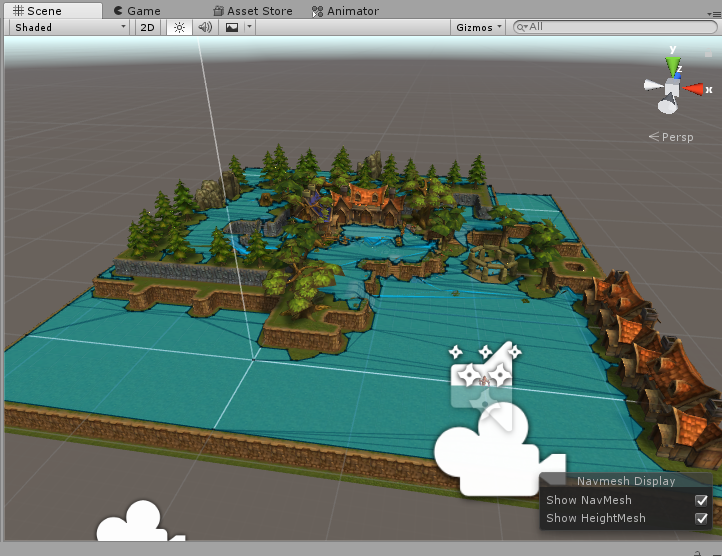
\includegraphics[width=0.4\textwidth]{Images/map.png}
    \caption{Generating the navmesh for the ennemy AI in Unity}
    \label{fig:navmesh_unity}
\end{figure}

\subsection{The interface}

We added an interface to give the player some feedback about what was going on using a unity canvas object facing the AR camera. We could see here the hero remaining health, the actual level and the selected spell thanks to a visual feedback in the top right corner of the screen (Figure \ref{fig:interface}).

\begin{figure}
    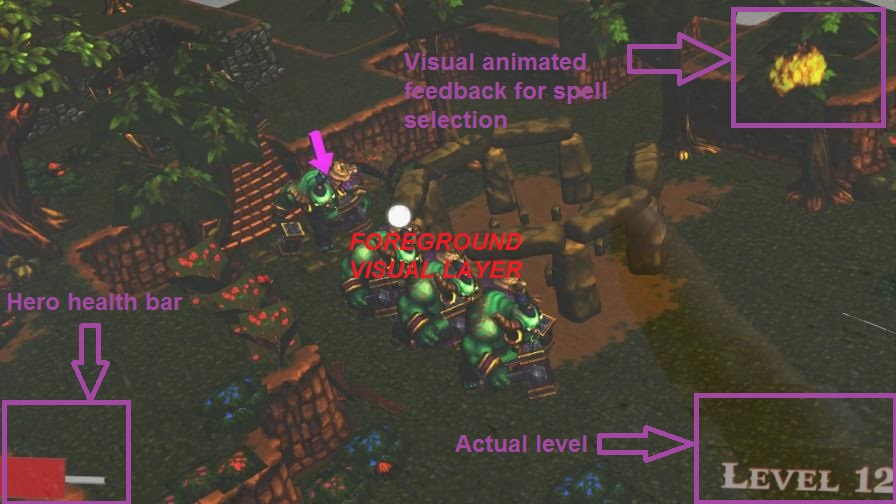
\includegraphics[width=0.4\textwidth]{Images/interface.jpg}
    \caption{A view of the interface and it's component from the user point of view}
    \label{fig:interface}
\end{figure}

\subsection{Animations}

The uncut animation files were also included in the assets provided. We needed to cut out the animations from the file provided, make state machines and triggers (see Figure \ref{fig:animation_state_machine}. Also, we needed to make additional triggers which would be used for enabling and disabling the weapon box colliders so they would cause damage only while the hit is ongoing instead of every time when the weapon collides with the player. This way we make the gameplay seem more natural even though we are not using the weapon box collider speed to determine should it cause damage or not. 

\begin{figure}
    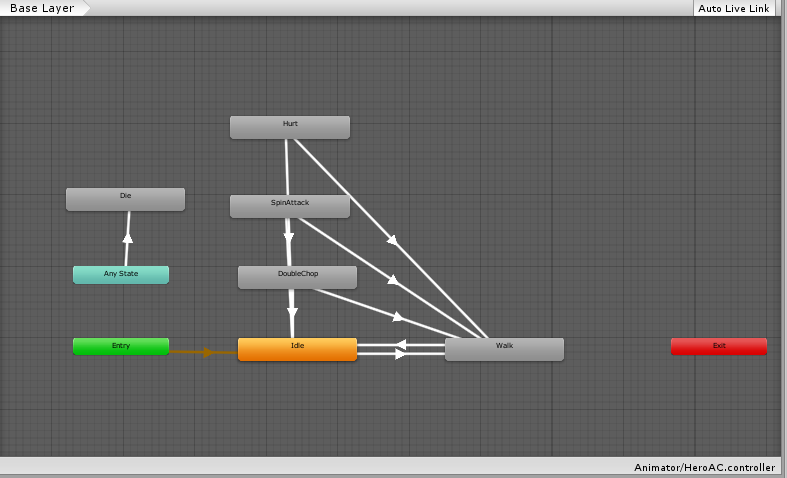
\includegraphics[width=0.4\textwidth]{Images/animation.png}
    \caption{Animation state machines in Unity}
    \label{fig:animation_state_machine}
\end{figure}

\subsection{Scripts}

GameManager – This script contains all game states and is in charge of spawning and killing enemies. It is also in charge of ending the game if the player dies or wins. The script implements the singleton pattern and is used by almost all of the other scripts to acquire and change game states.

EnemyAttack – This script takes parameters regarding the range within which the enemy should attack and time between two attacks. It checks is the player in range and triggers the attack if it is by playing the attack animation.

EnemyHealth – This script takes parameters regarding enemy starting health, the time since the last hit and the disappearing speed which determines when will the dead enemy sink trough the floor. If the enemy is dead it starts a timer for his disappearance.  It also contains the event handler for when the player sword collider enters the enemy collider and is in charge of deducting the enemy health and playing the hurt animation.

PlayerAttack – This script is similar to the EnemyAttack script – it takes the same parameters and it is in charge of checking are the enemies close enough. If they are, the script runs the “SpinAttack” animation of the hero and contains the event handler which enables the box collider on the hero’s swords in a specific moment of the animation. The box colliders are turned off the same way.

PlayerHealth – This script is quite similar to the EnemyHealth script. It has the event handler for the collision with the enemy weapons and the logic for taking hits and deducting the health. The main difference is the killPlayer() which differs from the killEnemy() from EnemyHealth.


\subsection{Spells and tangibles}

After putting aside the idea of making tangibles for traps, we still had to design the ones which would be used to create spells. Initially, the idea was to create a magical alphabet where each letter will be represented by a tangible. That way, the user could create from different letter combination magical words which will be the spells used later to attack enemies. That resulted in a set of 3 different letter and 2 different spells. See \ref{fig:letters} \ref{fig:fire} \ref{fig:lightning}.
\begin{figure}
    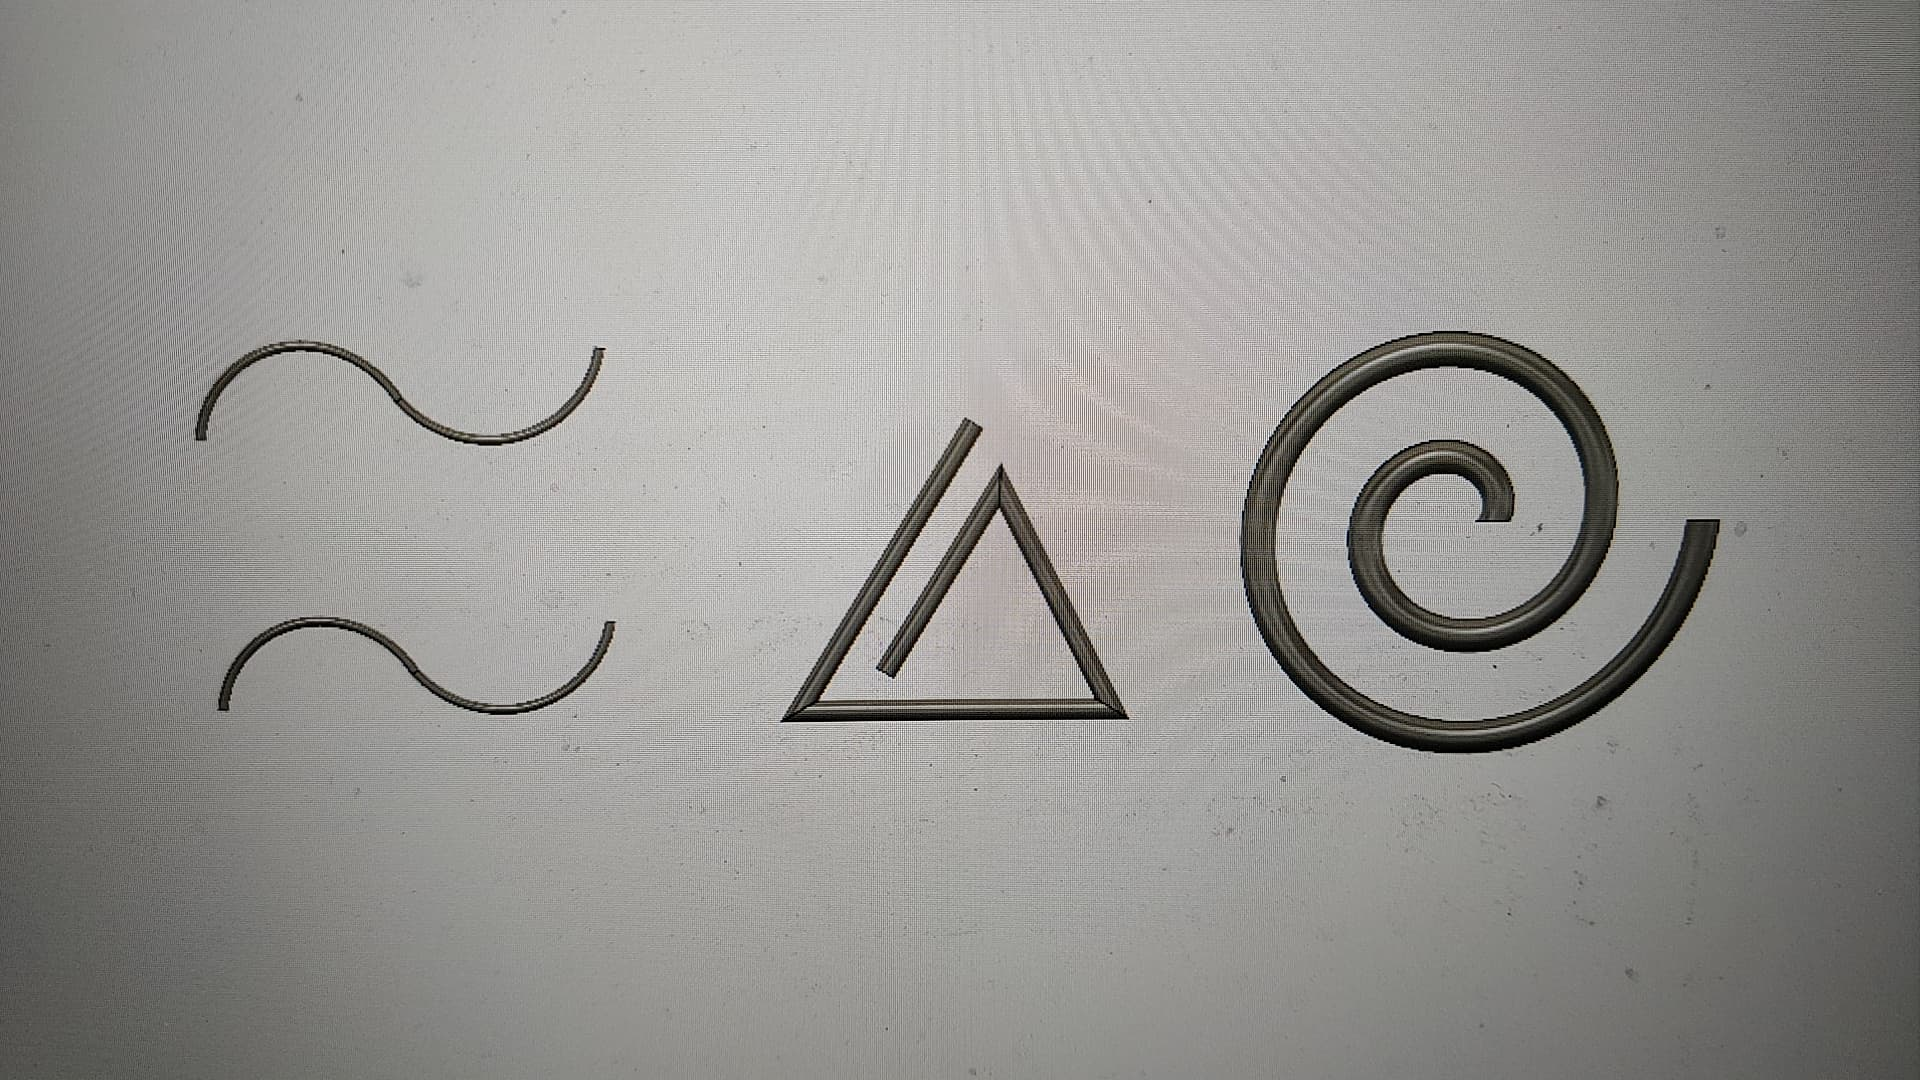
\includegraphics[width=0.4\textwidth]{Images/letter.jpg}
    \caption{Imaginary letter symbols used for creating each spell}
    \label{fig:letters}
\end{figure}

\begin{figure}
    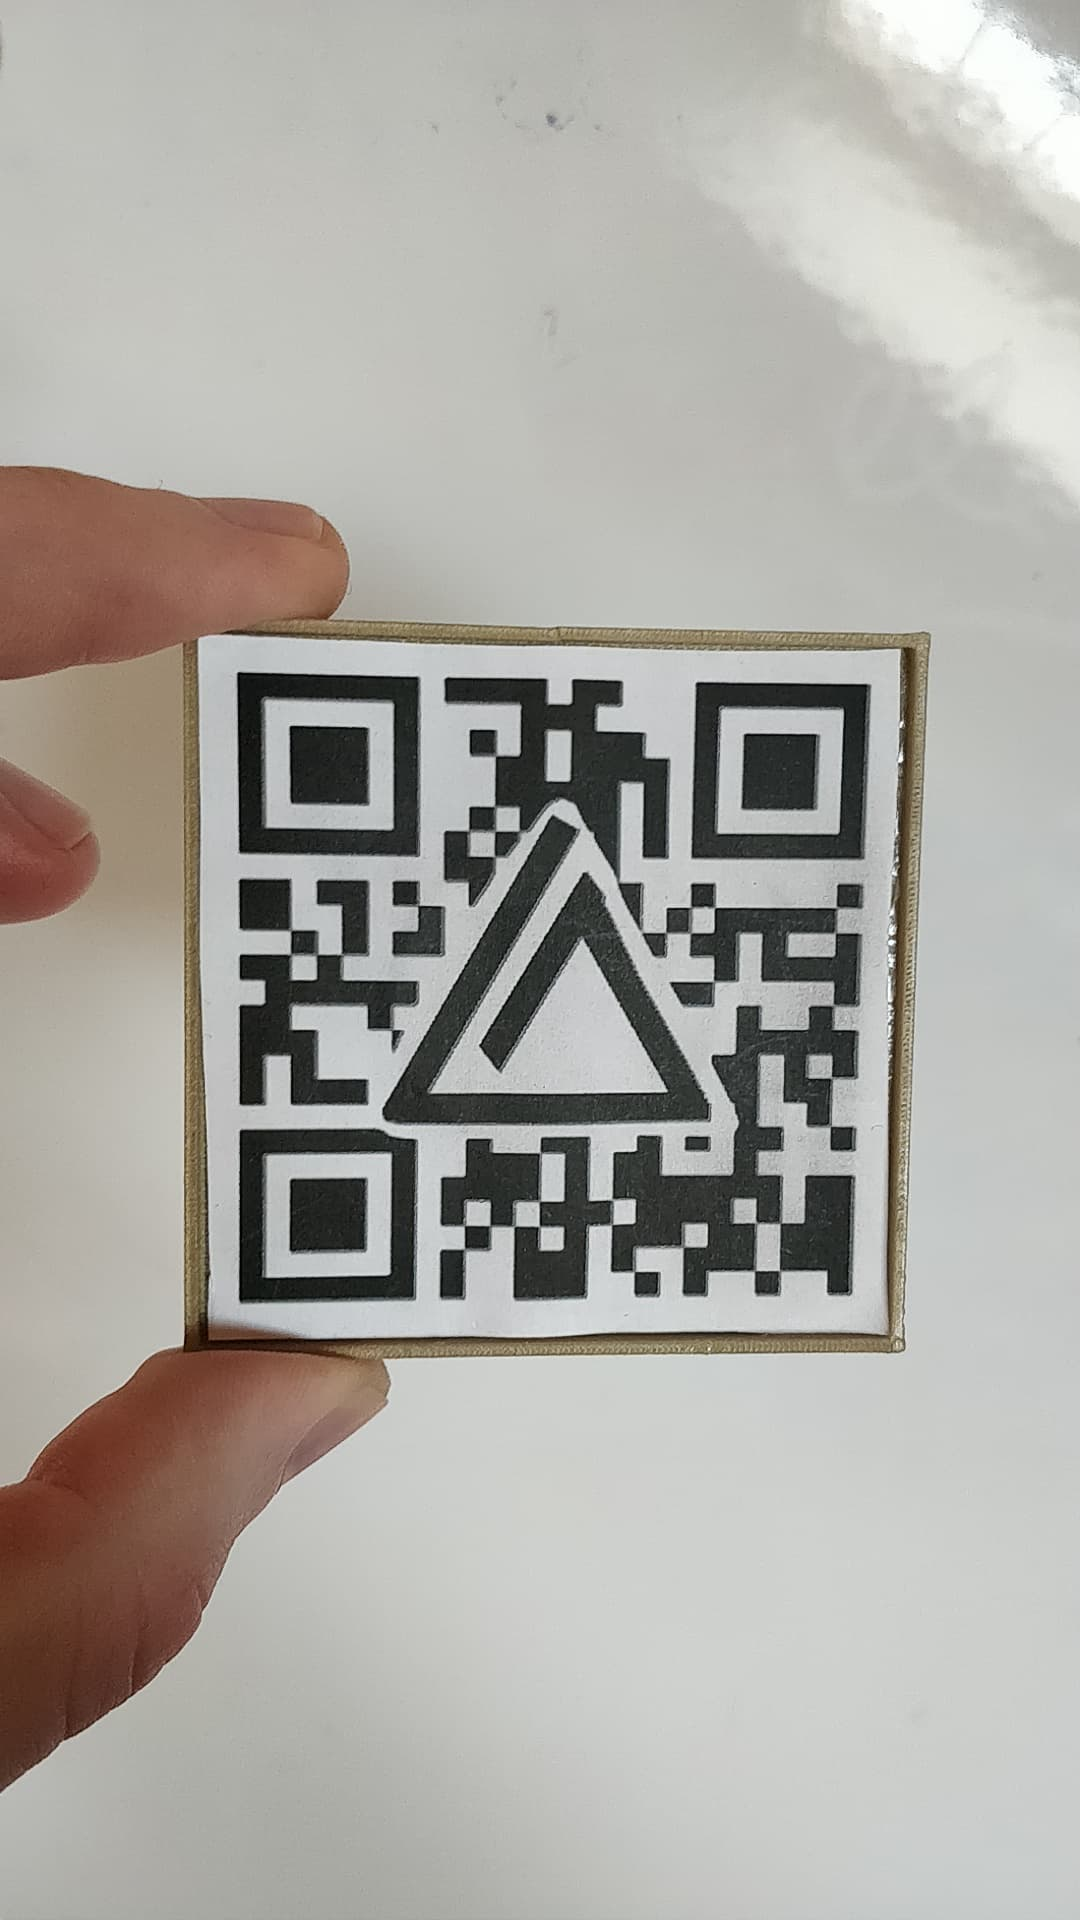
\includegraphics[height=0.4\textwidth]{Images/tangibleFront.jpg}
    \caption{Front of tangible marker used for the spell system, showing a marker}
    \label{fig:front_marker}
\end{figure}

\begin{figure}
    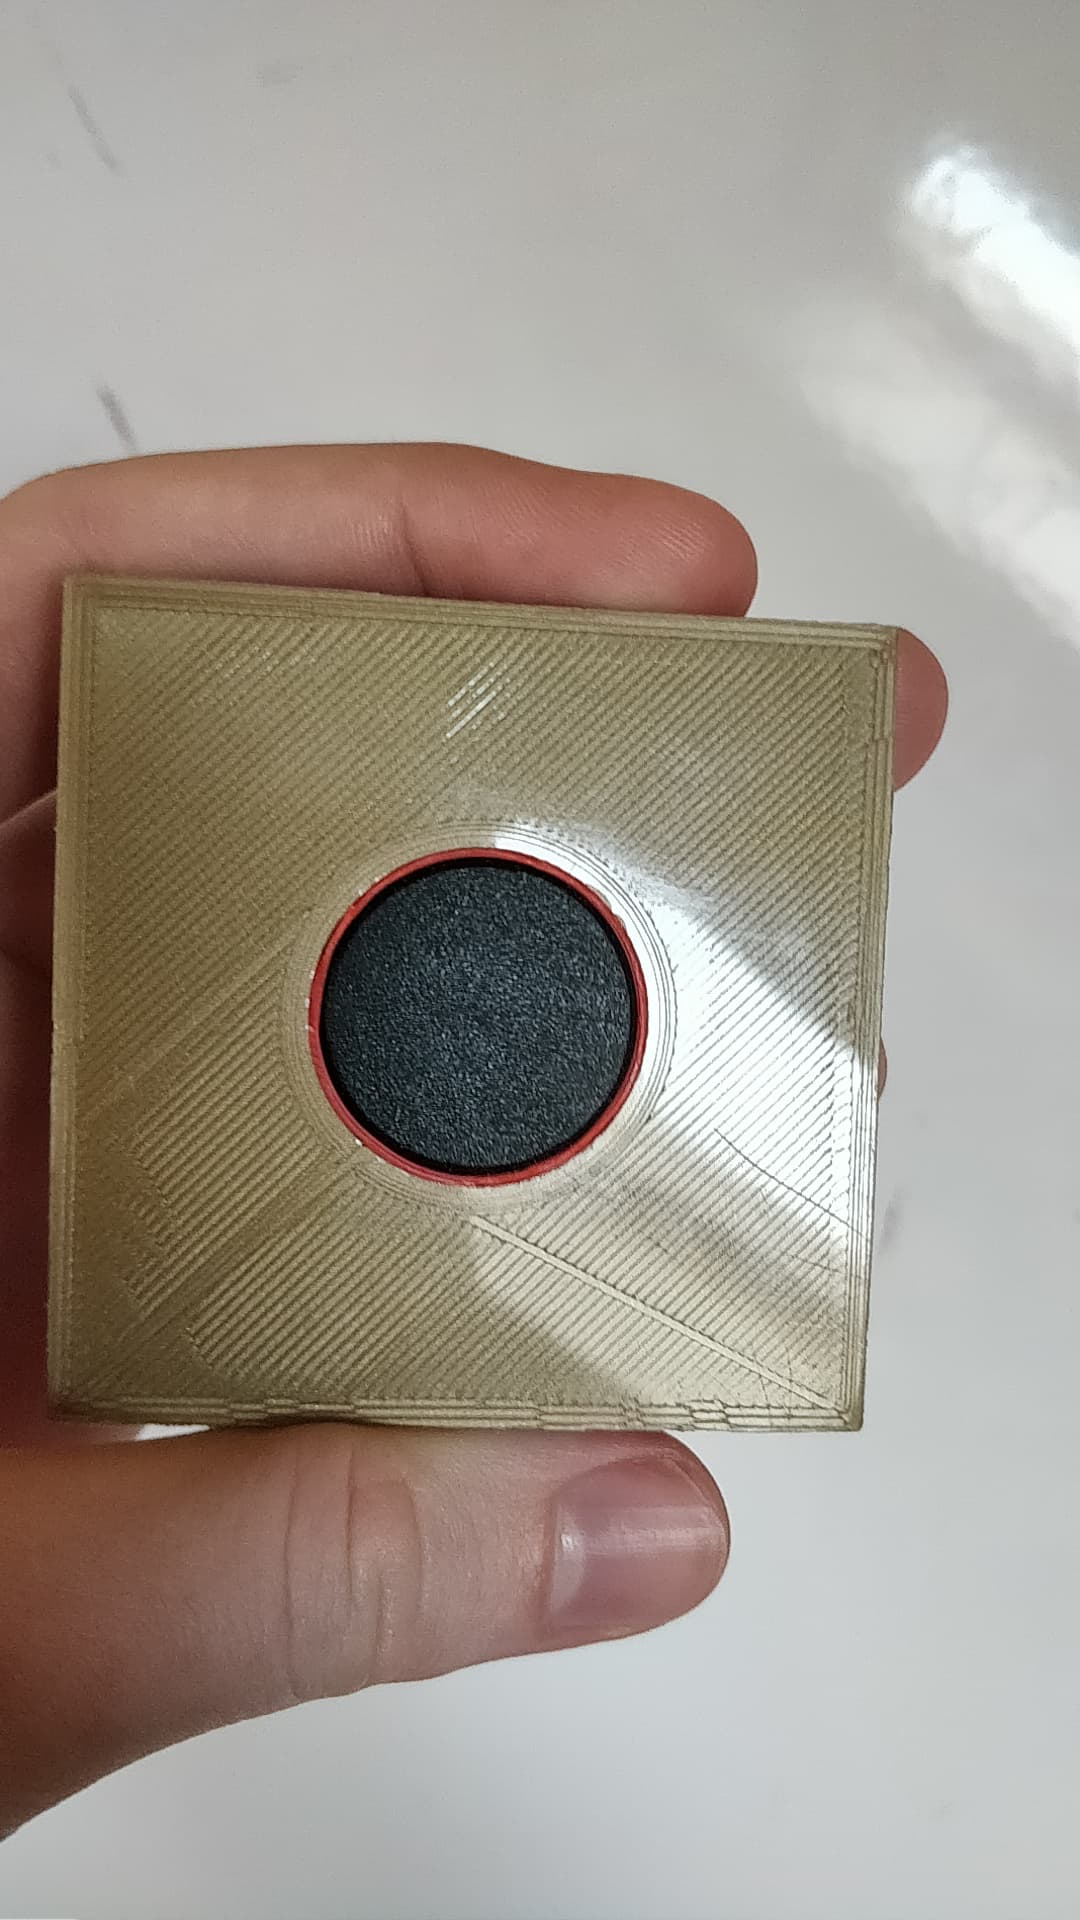
\includegraphics[height=0.4\textwidth]{Images/Tangibleback.jpg}
    \caption{Back of tangible marker used for the spell system showing the 3D printed casing and the magnet}
    \label{fig:back_marker}
\end{figure}

Once we were done with the theoretical part, we had to effectively design both the virtual object associated to this and the way the interact between each other, but also the tangibles and the way the user will interact with them.
For the virtual part, the letter floating above the tangibles were made using Fusion360 \cite{fusion360} and Unity. The image targets were made using Vuforia and the interaction between them (proximity detection, letter order) have been made using C\# scripts. The FX effect of fire and lightning have been made using unity free assets \cite{lightningbolts} \cite{unityparticles}.


Now comes the physical part of this design which involve how the user will interact with the spell’s tangibles. Thanks to one of our initial idea, we kept the painting palette as a support for the tangibles which will be not to exhaustive for the user to keep with him. The idea was to embed magnets inside the tangibles and a thin metal part inside the palette so the tangibles can be manipulated easily without falling when the user don’t need them. 

In the end, we used fridge magnets and a magnetic sheet which was glued on the palette to sustain the tangibles. Those ones were made in PLA using a 3D printer after having been designed using Fusion360. See Figures \ref{fig:front_marker} and \ref{fig:back_marker}. Finally, the image targets were made from modified QR codes to give some visual foreback about what will be displayed to the user. See Figure \ref{fig:marker_prototypes}.

\begin{figure}
    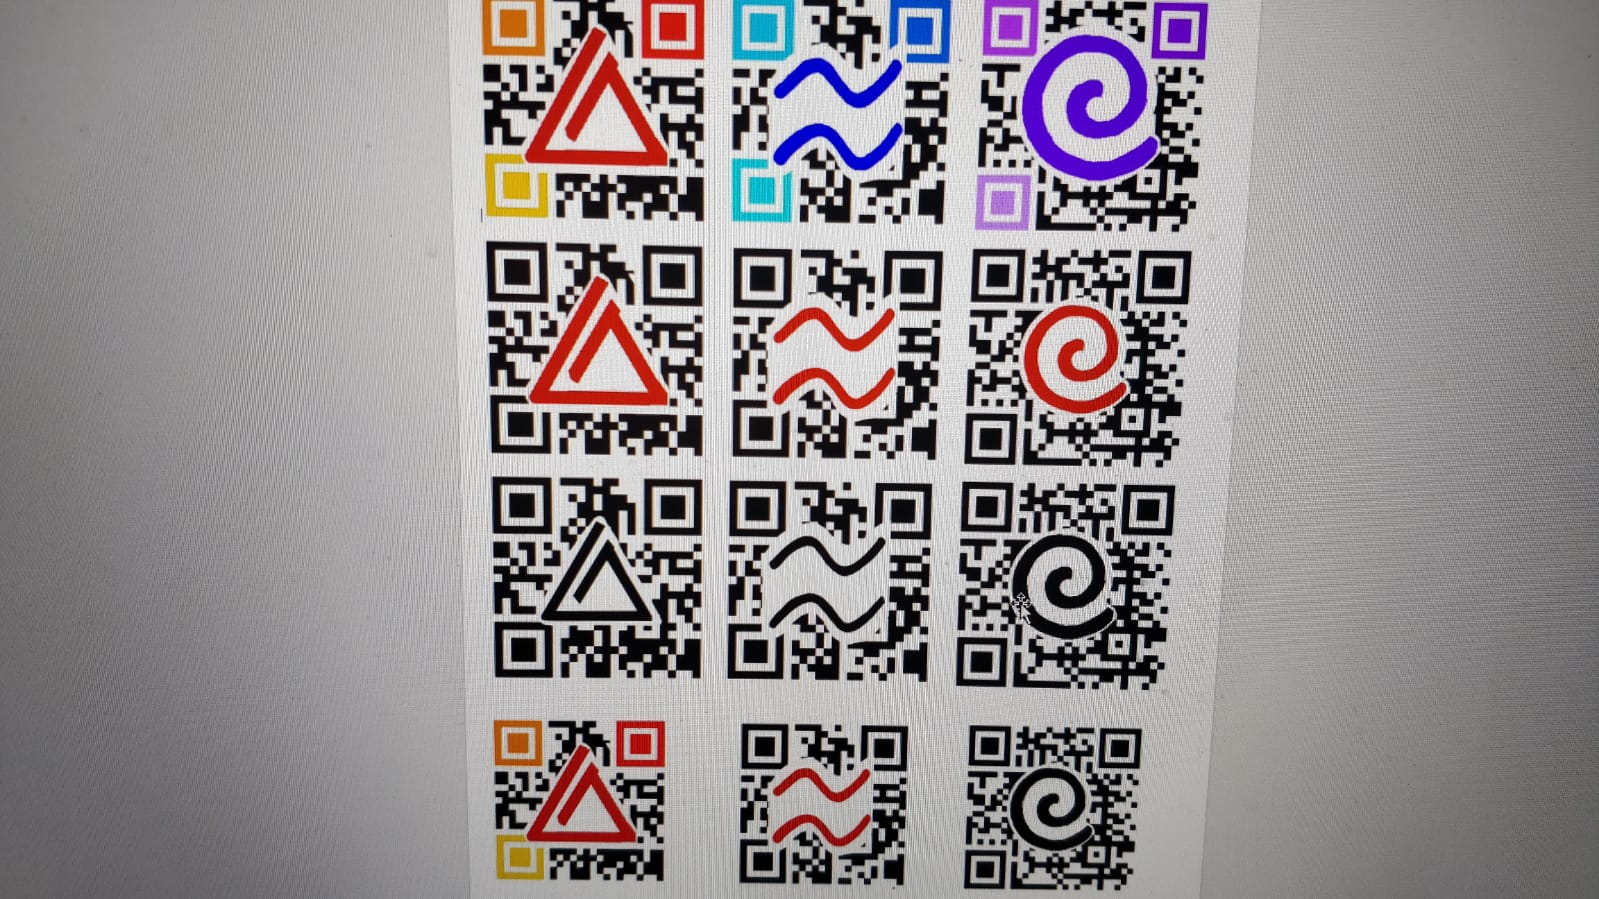
\includegraphics[width=0.4\textwidth]{Images/markers.jpeg}
    \caption{Prototypes of image target using modified QR codes to add visual feedback}
    \label{fig:marker_prototypes}
\end{figure}



\begin{figure}[ht]
 
\begin{subfigure}{0.5\textwidth}
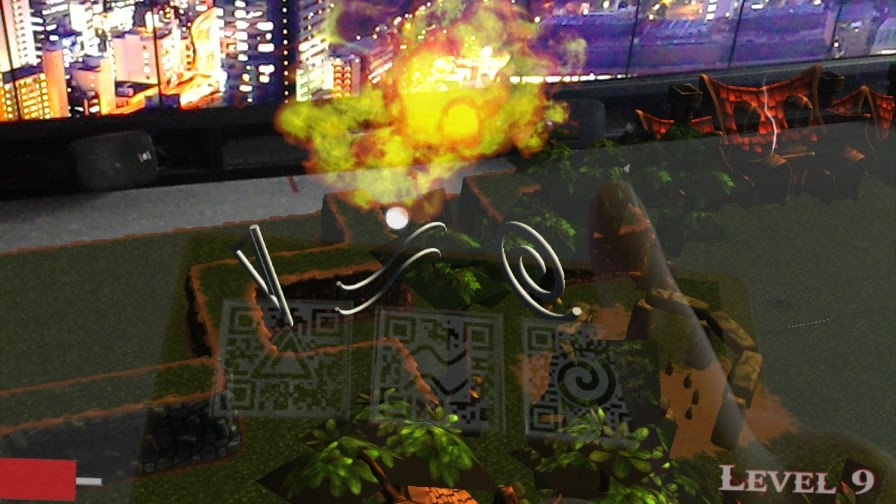
\includegraphics[width=0.9\linewidth, height=5cm]{Images/fire.jpg}
\caption{Fire formula combination}
\label{fig:fire}
\end{subfigure}
\begin{subfigure}{0.5\textwidth}
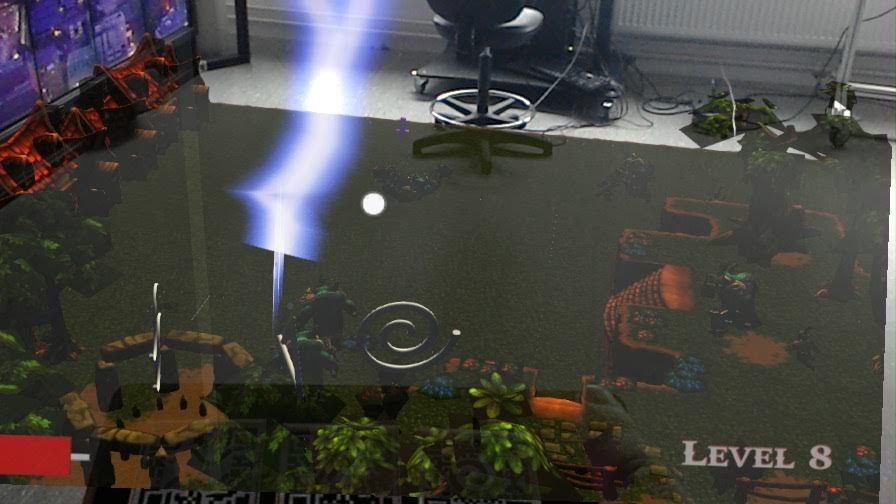
\includegraphics[width=0.9\linewidth, height=5cm]{Images/lightning.jpg}
\caption{Lighting formula combination}
\label{fig:lightning}
\end{subfigure}
 
\caption{Combination of the letter to create the different spells captured through AR device Hololens view}
\label{fig:spell_combinations}
\end{figure}




\subsection{Hololens}


Creating apps for the Hololens was made easier by the fact that both Unity and Vuforia had tools compatible with it. A well known framework is the Mixed reality toolkit \cite{mixedtoolkit} developed toolkit which makes development of mixed reality apps for different devices (including Hololens) easier. Unfortunately we couldn’t make it work with the Unity version we had been working with, but it was used as a reference during the development of the app. The Mixed Reality Academy \cite{microsoft-academy} tutorials by Microsoft was also used extensively.

The Hololens has advantages over mobile phone AR, because it is a computer mounted on a users head. This means more computing power, hands free immersion, similar to VR headsets but without needing cables linked up to a stationary computer. 



\section{Evaluation}
% Observation during the exhibition, difficulties noticed by yourself

Even if the only kind of evaluation we were able to do was to get some feedback during the exhibition directly after people had played the game, we have fought of 3 main points that could lead us to improvements : the immersion, the tangible design and the gameplay itself.

We know that one of the most important point when you use AR or VR is the immersion factor. It depends of many different variables which allow the user to dive into the game and enjoy the experience. We tried as much as possible to play with this using sounds, music, making the landscape look like a real video game, and trying to reduce as much as possible the presence of the real room behind the virtual scene. Those factors could lead to some experiments, trying to get the game as immersive as possible in finding the best settings for the user.

It could have been also nice to run some more experiments with the tangibles and the palette shape to ensure the most suited tracking for the Hololens as well as reducing the fatigue of the user as much as possible. That also mean testing different image target size and color (something we have done at a small extent) in order to maximize the efficiency of the marker tracking side of our system.

Lastly, we could evaluate the gameplay itself to see how satisfying playing this game is for the users, in particular if the use of tangibles is really a fun mechanic that matters or if it’s just a constraint for them.



\section{Results}
% feedback during the exhibition

As said before, this part is mainly about the feedback we had from people after playing the game and what we observed while they were playing. 

The first thing that we observed was that a tutorial to explain what will happen would have been really nice because our explanations were not perfect plus it was breaking the immersion. For instance we had to help the user many times while they were trying to manipulate the tangibles to create spells or to differentiate the hero they had to defend from the enemies attacking him. People were also not used to the fact that they could move in the room to move around the map and change their point of view or even crouch down to target the enemies more easily even if some people did that naturally. 

But one of the main problem was the pinching gesture from the Hololens which is, if you’re not used to it, really hard to perform preventing some to even play the game because they were not able to select spells. Some even tried different gestures (grabbing the spell, drag and drop it) to interact with the virtual object according to one of our initial idea for this project. This was really interesting showing once again that the pinching gesture is not really meaningful in this situation.

Another problem related to this was the fact that people didn’t always understood that the gaze and the gesture were not directly related, meaning that you don’t have to do the pinching gesture exactly where you’re gazing to make it work. Some even thought that the spell needed to always be displayed on the screen for it to work and kept holding the palette in front of them.

This could be linked to one main problem which was caused by the Hololens technology which give a really small field of view for marker tracking and it was sometime hard to get the three needed markers as well as the spell FX on the same screen, making the selection again more complicated for the user.
The way the painting palette as to be held was also not something usual and many people did not understood how to keep it in their hand without being annoyed. 

Overall people really enjoyed the system and playing the game. We had been told many times that the scene quality was good even comparing it to the very popular Warcraft III game \cite{warcraft}, making it way more enjoyable and showing once again that the graphic quality of the game really matter. People also liked the fact of using recipes to make spells and being able to manipulate them physically even if the tracking was problematic. But once one get used to the pinching gesture and the game mechanics, they had a lot of fun playing and watching enemies exploding from above.



\section{Challenges}

In order to get to the end of the project, we had to face many challenges mainly due to the technology we wanted to use, in particular the Hololens. The low angle of vision was definitely a drawback to track tangibles that are used at arms length, questioning our initial ideas. We managed to get through it, shaping the size of the image target as small as possible without losing too much tracking power resulting in a size of 6*6cm for each image target. 

We also had a lot of troubles on the software side of the project because even if Unity was the center piece of the project, linking it with the good version of both Vuforia and all the Hololens requirements was a real nightmare. We also took a lot of time to test each of our feature on the Hololens because the procedure to do it was really long (two builds each time !)


\subsection{Future works}

A big feature we wanted to implement was occlusion. Parts of the scene should be hidden if real world objects are in the way, increasing immersion further. Improving the design of all the tangibles was also something we wanted to achieve but the lack of time resulted in something which was satisfying but still basic.

Having tangibles that could be directly set up in the map, for traps and obstacles, would be very interesting to expand the gameplay, and very similar to what we already have in the system. The tricky part being to have a kind of persistence in the environment about the object.

We only explored a small subset of the features and tools the Hololens offers. Spatial mapping and spatial sounds could be explored to enhance the immersion of the player, and also help setup the map for a better overall experience. 

Adding gestural interaction with external sensors could help interact with the spells and the game using Myo’s or smartphones attached to the arm. It will also for a wider ranged of gestures and especially for gestures without having to rely on the cameras short field of view.

The spells interaction work, selecting the spell could be made more natural by replacing the tapping movement by something closer to “holding” the spell. More markers could be make to create more spells, different types of combinations could be made to improve on the set of actions and gameplay. An idea was to move away from markers and using something like NFC technology to detect tangible proximity, again to counter the Hololens short field of view.

Gameplay is also improvable, ideas include : multiplayer (cooperative gameplay for example), adding systems to make spells discoverable (spell books, physical or virtual), more types of enemies, procedurally generated maps, etc.

The Hololens 2 is supposed to be coming out this year, hopefully with a bigger field of view for the cameras and bigger screens to help track objects close to the user.

\begin{figure}
    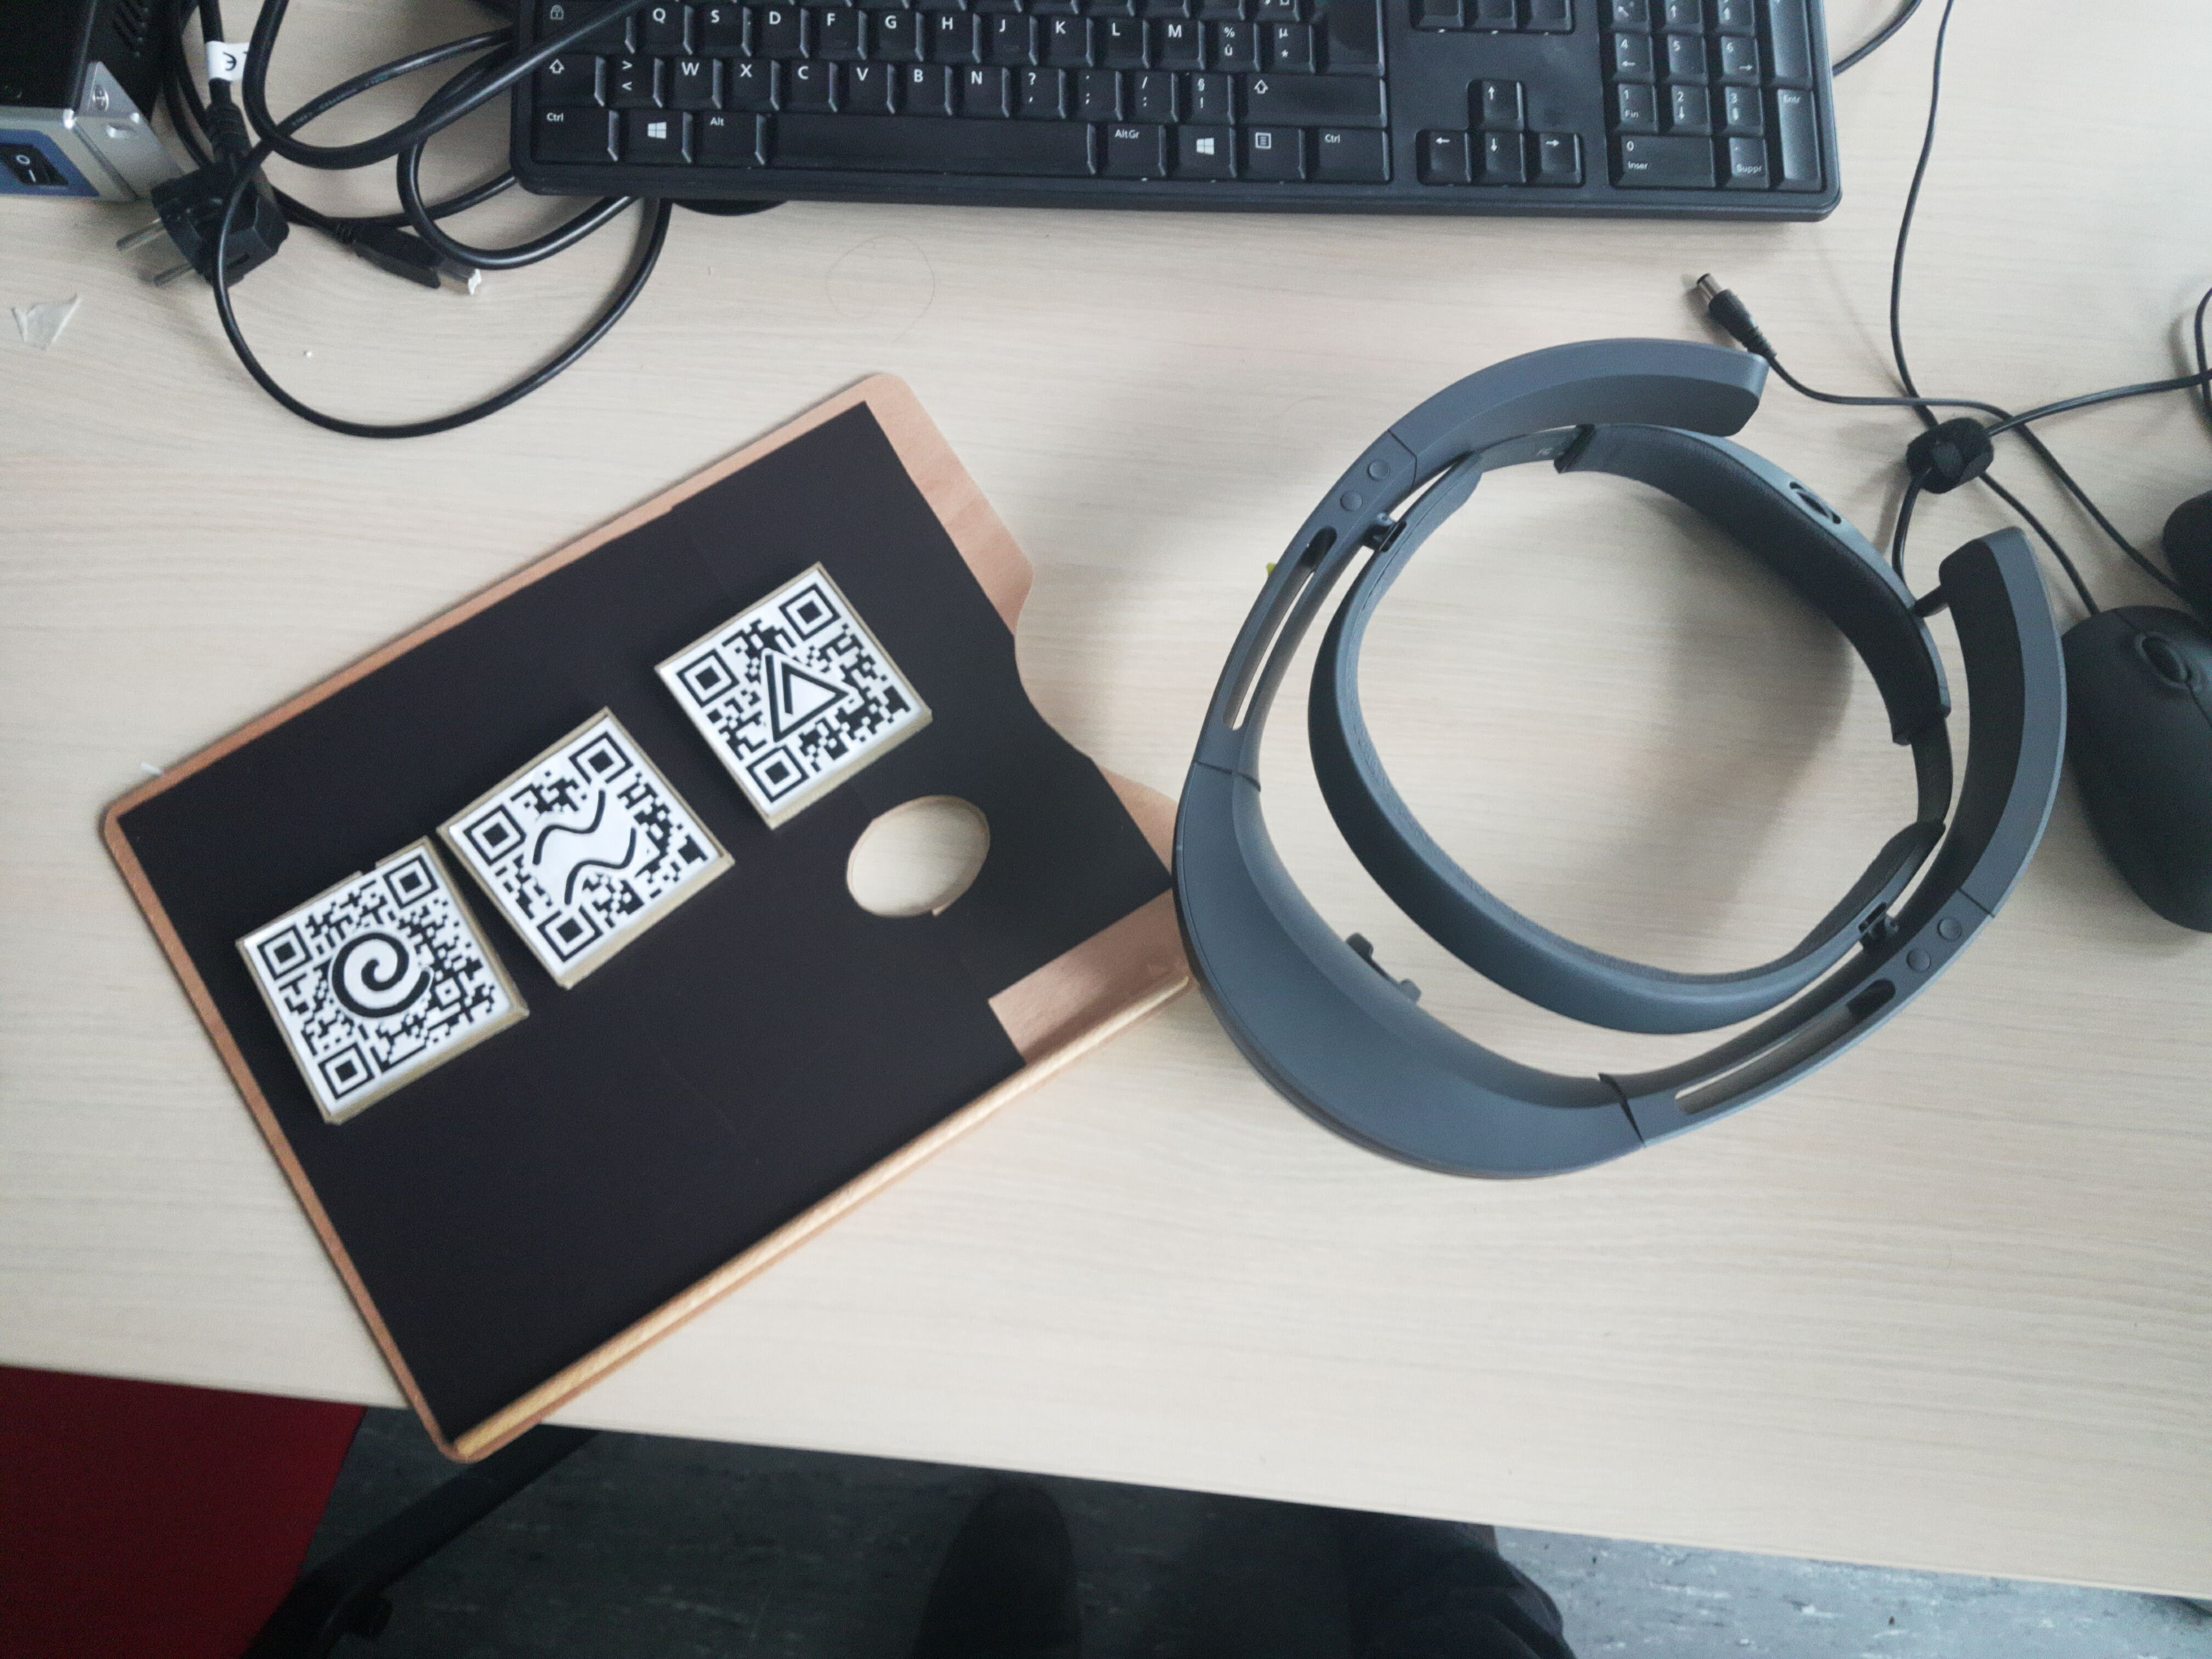
\includegraphics[height=0.35\textwidth]{Images/tangibles+helmet.jpg}
    \caption{Closeup on the tangibles, the palette to use them on and the helmet. The AR Spells doesn't require much material wise.}
    \label{fig:tangibles_helmet}
\end{figure}

\section{Conclusion}

We presented AR Spells, an augmented reality game that combines the Hololens with tangible markers to create an immersive game experience. We have shown that tangibles and augmented reality work well together in creating an immersive experience for the user. Many improvements are still possible for our design, but a lot of the technology is already here and needs to be combined and explored to create even more imaginative systems. Once augmented reality headsets become more affordable, creating games and sports with those technologies are going to be more popular. We believe that moving away from traditional interfaces seen in video games for those types of applications is key to making immersive, enjoyable augmented reality games in room-sized environments.

%
% The acknowledgments section is defined using the "acks" environment (and NOT an unnumbered section). This ensures
% the proper identification of the section in the article metadata, and the consistent spelling of the heading.
\begin{acks}
We would like to thank the following people :
\begin{itemize}
    \item Anastasia Bezerianos for allowing use to use the Hololens and giving us access to the lab to use it
    \item Jean-Marc Vezien for his showing of episode 1 of Denou Coil which sparked some of the initial ideas
    \item Olivier Gladin for babysitting us in Digiteo's WILDER room while we developed on the Hololens
    \item Rafael James for his numerous help with Vuforia and the Hololens and helping in making everything work together
    \item Romain Di Vozzo for managing Digiteo's Fablab and helping out with the 3D printers for the tangibles
\end{itemize}
\end{acks}

%
% The next two lines define the bibliography style to be used, and the bibliography file.

\bibliographystyle{plain}
\bibliography{arspells}


\end{document}
